%author: ouyang
%compile: pdflatex

\documentclass[cjk,slidestop,mathserif]{beamer}

%\usepackage[utf8]{inputenc}
%\usepackage{default}
%\usepackage{xcolor}
\usepackage{CJK}
\usepackage{graphicx}
%\useoutertheme{infolines}%将作者名字和页码标下来,但是还是没有运行出来 
%\usecolortheme{default}
\useoutertheme{infolines}
%\usetheme{umbc1}	%这个东西因为不是内嵌的,所以最后没成功,查阅?????
\usetheme{Warsaw}	%在rochester情况下面,可以现实页码,但是如果将其该改成了warsaw,则就显示不了了,可能是具体设置的问题
\usecolortheme{crane} %others whale, seahorse,dolphin
\usecolortheme{seagull} %orchid, lily

\setbeamertemplate{items}[ball]%把item枚举出来的作为圆!还有一个enumerate,可以是1,2,3等!!!

\setbeamertemplate{blocks}[rounded][shadow=true]%这个地方只是使用定理时,矩形区域才是有阴影的
\setbeamertemplate{navigation symbols}{}%去除底部比较酷的工具条,因为实际应用的很少
%\setbeamertemplate{footline}%[frame number]%这里是为每页的最下面加上页码号!!!这个的作用!!!

\begin{document}
\begin{CJK}{UTF8}{gkai}
\title{Ceph: A Scalable, High-Performance Distributed File System}
\author{Sage A. Wei, Scott A. Brandt etc.}
\institute[HUST]{University of California, Santa Cruz}
\date{\today}
\frame{\titlepage}%划分,到这里为止,就是第一页的显示
 
%to declare the contents before every chapter
\AtBeginSection{
\begin{frame}{contents}
 \tableofcontents[currentsection, hideallsubsections]
\end{frame}
}

\frame{\tableofcontents}%这个东西的作用就是将subsection的东西啥的列做目录
\section{Motivation}
\begin{frame}
 \frametitle{Background and Present situation}
 \begin{exampleblock}{Key Point}
 The performance of file system have proved critical to the overall performance of tremendous APPs.  \\
 
 Since system designers have long sought to enhance the performance and scalability of distributed storage systems (DFS).
  \end{exampleblock}
  
  \textbf{Present Solutions}:
  \begin{enumerate}
   \item NFS, sever exports a file system hierachy that clients can map into their local namespace, \alert{limited} to C/S model obstacle.
   \item OSD storage, Clients interact with metadata server of metadata oper. and OSDs of file I/O, scalability improved, \alert{limited} little or no distribution of metadata workload. 
  \end{enumerate}
\end{frame}

\begin{frame}
 \frametitle{Design Goals}
 \vspace{8pt}
 Then Ceph, a scalable and high-performance DFS, is presented under such circumstances. There are two points of creations:
 \begin{itemize}
  \item[**] Decouples data and metadata operations, replacing file allocation tables with Generating functions (CHRUSH).
  \item[**] A high adaptive distributed metadata cluster architecture, scalability improved.
 \end{itemize}
 \vspace{4pt}
\alert{Assumption}: Systems at the petabyte scale are inherently dynamic.
\end{frame}

\section{Ceph's Structure}
\begin{frame}
 \frametitle{System's Overview}
 \vspace{6pt}
 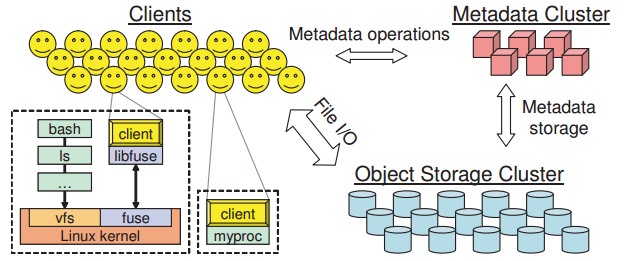
\includegraphics[width=\textwidth]{p1.png} \\
 Ceph system has three main components: clients (near-POSIX file system interface), 
 a cluster of OSDs (store all data and metadata), 
 a metadata server cluster(MDS) (namespace, security, consistency and coherence). 
\end{frame}

\subsection{Clients}
\begin{frame}
 \frametitle{File I/O and Capabilities}
 \vspace{12pt}
 When a process \textbf{opens} a file, the clients \textbf{sends} a request to MDS cluster. 
 then MDS \textbf{translate} it to the file inode, if it \textbf{exists}, the access is granted. \\
 
 \vspace{8pt}
 Ceph has lots of striping strategies to \textbf{map} file data onto a sequence of objects, and objects names simply 
 combine the \textbf{file inode num.} and the \textbf{strip number}. And objects replicas are assigned to OSDs using CRUSH (a 
 global mapping function).
\end{frame}

\begin{frame}
 \frametitle{Client Synchronization}
 \vspace{4pt}
 When a file is \textbf{open}ed by multiple clients with either \textbf{multiple writers} or a \textbf{mix} of readers and writers,
 MDS \textbf{revoke} any previously read caching and write buffer, \textbf{force} client I/O be synchronous. \\
 \vspace{4pt}
 Each APPs read or write \textbf{operations} will \textbf{block} until is acknowledged by the OSD, making the burden \textbf{serialization}, 
 and objects are also to ultilize for \textbf{large writes} by acquring \textbf{locks}. \\
 \vspace{4pt}
 Indeed, synchronous I/O can be a performance \textbf{killer} for APPs, So it is often desirable to \textbf{relax consistency} sometimes,
 and Ceph supports such relaxation via a \textbf{global switch}.
 
 \vspace{4pt}
 \textbf{What's more} Ceph has acheived a set of POSIX I/O interface, eg. O\_LAZY etc.
\end{frame}

\begin{frame}
 \frametitle{Namespace Operations}
 \vspace{6pt}
 Clients interact with the DFS \textbf{namespace} by the \textbf{MDS}. And Ceph \textbf{optimizes} for the most common metadata access scenarios,
 \textbf{eg}. $readdir$ followed by a $stat$ of each file ... \\
 \vspace{4pt}
 Ceph could allow consistency to be further \textbf{relaxed} by caching metadata \textbf{longer}, like the NFS for $30$s. \\
 \vspace{4pt}
 Issues stated above may \textbf{break} coherency, so Ceph addresses such problem by revoking any write capabilities 
 to momentarily \textbf{stop} from all writers, the highest values are returned with the $stat$ reply.\\
 \vspace{4pt}
 Although the stop is dramastic, but it is \textbf{essential to serialization}.
\end{frame}

\subsection{Metadata Servers cluster (MDS)}
\begin{frame}
 \frametitle{About the Metadata}
 \vspace{8pt}
 \begin{exampleblock}{A Fact}
  Metadata oper. often makes up as much as half of file system workloads and lie in the critical path, 
  making the MDS cluster critical to overall performance.
 \end{exampleblock}
  \vspace{4pt}
  File and directory metadata in Ceph is very small, object names constructed using inode number, and distributed 
  to OSDs using CRUSH, which has \textbf{advantages}.
\end{frame}

\begin{frame}
 \frametitle{Metadata Storage}
 \vspace{8pt}
 A set of large, bounded, lazily flushed \textbf{journals} allows each MDS to quickly \textbf{stream} its updated metadata 
 to the OSD cluster in an efficient and distributed \textbf{manner}.\\
 \vspace{4pt}
 %MDS recovery is not yet implemented, whereas journals are designed such that in the event of a MDS failure, 
 %another node can rescan the journal to recovery the critical contents of the failed node, then recover the 
 %file system state.
 Such strategy provides streaming updates to disk in an \textbf{efficient} fashion, and a vastly \textbf{reduced} re-write workloads.\\
 \vspace{4pt}
 Besides, inodes are embeded within directories, allowing the MDSs to \textbf{prefetch} entire directories with a \textbf{single} 
 OSD read request.
\end{frame}

\begin{frame}
 \frametitle{Dynamic Subtree Partitioning}
 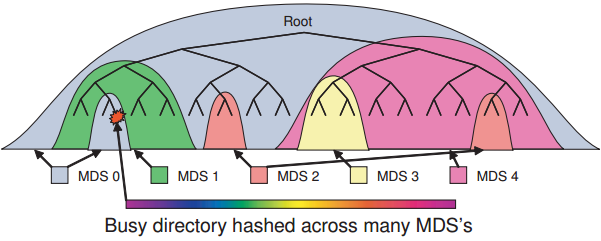
\includegraphics[width=\textwidth]{p2.png} \\
 Background (Static subtree partition and harsh table), then Ceph is based on a dynamic subtree partition 
 strategy.\\
 \vspace{2pt}
 Ceph dynamically \textbf{maps} subtrees of the directory hierachy to metadata servers \textbf{based on} the current workload. 
 
\end{frame}

\begin{frame}
 \frametitle{Dynamic Subtree Partitioning}
 \vspace{12pt}
 Each MDS measures the \textbf{popularity} of metadata using counters with time decay. Any \textbf{operations} 
 \textbf{increments} the counter on the affected inode and all its ancestors up to the directory. \\
 \vspace{6pt}
 And each MDS has a \text{weighted tree} describing the recent workload distribution, and appropriated-sized 
 subtrees are \textbf{migrated} to keep 
 the workload evenly distributed (sharing namespace locks).
\end{frame}

\begin{frame}
 \frametitle{Traffic Control}
 \vspace{6pt}
 Such strategy can balance a broad range of workload, but can not always cope with \textbf{hot spots} or \textbf{flash crowds}. 
 So Ceph uses its knowledge of metadata popularity to provide a \textbf{wide distribution} for hot spots.\\
 \vspace{4pt}
 \begin{itemize}
  \item[*] \textbf{read} directories are replicated across multiple nodes to distribute load.
  \item[*] \textbf{write} workload have their contents hashed by file name across the cluster, a balanced distribution while locality expense.
 \end{itemize}
  Every MDS \textbf{response} provides the client with updated information, allowing them to know what has occurred with their interaction.
\end{frame}

\subsection{Object Storage Devices cluster(OSDs)}
\begin{frame}
 \frametitle{overview OSDs}
 \vspace{18pt}
 From a high level, Ceph clients and MDS view the OSDs cluster as a \textbf{single} logical object store and namespace. \\
 \vspace{6pt}
 Ceph's Reliable Autonomic Distributed Object Store(RADOS) acheives linear scaling in both capacity and aggregate performance 
 by management of \textbf{object replication}, \textbf{cluster expansion}, \textbf{failure detection}, and \textbf{recovery to OSDs}.
\end{frame}

\begin{frame}
 \frametitle{Data Distributed with CRUSH}
 \vspace{12pt}
 Now Ceph must distribute data among a cluster of thousands of storage devices so that device storage and 
 bandwidth resouces are effectively ultilized, but there comes a problem, \alert{how to avoid imbalance?} \\
 \vspace{6pt}
 %\pause
 Ceph's \textbf{strategy}: \\
 \begin{itemize}
  \item firstly, map objects into placement groups(PGs) using simple hash function.
  \item then, PGs are assigned to OSDs using CRUSH(controlled replication under scalable hashing \ldots).
 \end{itemize}
\end{frame}

\begin{frame}
 \frametitle{Data Distributed with CRUSH}
 \vspace{6pt}
 To \textbf{locate} any object, CRUSH requires only the PG and an OSD cluster map.\\
 such approach has two key \textbf{advantages}:\\
 \begin{enumerate}
  \item completed distributed, then any party can independently caculate the locatin of any object;
  \item map infrequently updated, eliminating any exchange of distribution-related metadata.
 \end{enumerate}
 \vspace{4pt}
 CRUSH maps PGs onto OSDs based on \textbf{placement rules}, which define the level of replication and any constraints on placement.
\end{frame}

\begin{frame}
 \frametitle{Data Safety}
 \vspace{18pt}
 In DFS, there are two reasons why data is written to \textbf{shared storage}:\\
 \begin{itemize}
  \item[*] clients are interested in making their updates visible to other clients;
  \item[*] clients are interested in knowing that the data they've written is safely replicated.
 \end{itemize}
\vspace{4pt}
Then Ceph realizes both low-latency updates for efficient APPs synchronization and well-defined data safety semantic.
\end{frame}

\begin{frame}
 \frametitle{Data Safety}
 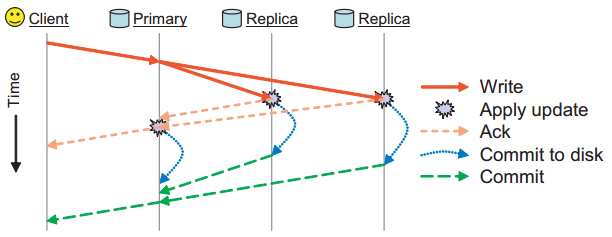
\includegraphics[width=\textwidth]{p4.png} \\
 Ceph responds with an $ack$ after the write has been applied to the buffer caches on all OSDs replicating the objects.\\
 \vspace{4pt}
 By default, clients also \textbf{buffer} writes until they commit to avoid data loss in the event of a similtaneous power loss to all OSDs	in the PG.
\end{frame}

\begin{frame}
 \frametitle{Replication and Failure Detection}
 \vspace{6pt}
 \begin{columns}[c]
    \column{0.5\textwidth}
    \textbf{Replication}: \\
    Data is replicated in terms of PGs, each of which is mapped to an ordered list of $n$ OSDs(for $n$-way replication).
    \column{0.5\textwidth}
    \textbf{Failure Detection}: \\
    Ceph's \textbf{failure} has two types: one is disk error or corrupted data, which OSDs can self-report; 
    the other is an OSD unreachable on the network, which requires active monitoring. \\
    \vspace{4pt}
    ODS \textbf{liveness}: an unresponsible OSD is marked $down$, and if the OSD does not quickly recover, it is marked $out$.
 \end{columns}
\end{frame}

\begin{frame}
 \frametitle{Recovery and Cluster Updates}
 OSD failure, recoveries etc. will \textbf{change} the OSD cluster, Ceph will change such changes \textbf{in the same way}. 
 And so Ceph maintain a \textbf{version number} for each object and a \textbf{log} of recent changes for each PG. \\
 \vspace{2pt}
 When an active OSD receives an \textbf{updated} cluster map, then \\
 \begin{enumerate}
  \item iterate over all locally stored PGs and CRUSH mapping to determine the primary and replica.
  \item if PG has changed, the OSD peers with the PG's other OSDs.(collect info., verify it, then send to all the OSDs).
  \item OSDs are then independently responsible for retrieving missing or outdatad objects from their peers.
  \item OSD delays processing any request for a stale or missing object.
 \end{enumerate}
\end{frame}


%\begin{frame}
% \frametitle{Object Storage with EBOFS}
% 
%\end{frame}

\section{Evaluation}
\begin{frame}
 \frametitle{The Tests' platform}
 \vspace{12pt}
 \begin{exampleblock}{Platform}
  Clients, OSDs and MDSs are user processes runing on a dual-processor Linux cluster with SCSI disks, TCP communication. OSD or MDS own host, while clients share the same host generating workloads.
 \end{exampleblock}
 \begin{exampleblock}{Goals}
  To demonstrate Ceph's \textbf{performance}, \textbf{reliability} and \textbf{scalability}, focusing on Data and Metadata performance.
 \end{exampleblock}
\end{frame}

\subsection{Data Performance}
\begin{frame}
 \frametitle{OSD Throughput and Write Latency}
 %\vspace{2pt}
 \begin{columns}[c]
    \column{0.5\textwidth}
  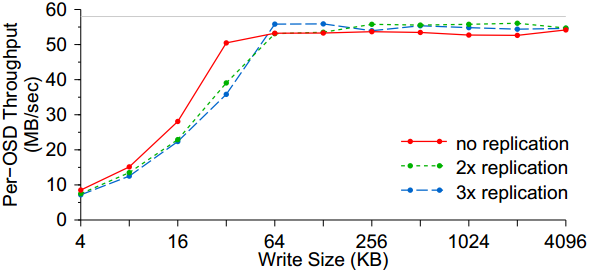
\includegraphics[width=\columnwidth]{p5.png} \\
  %Per-OSD write performance. 
  \begin{enumerate}
   \item horizontal line, upper limit imposed by the physical disk.
   \item Replication has minimal impact on OSD throughput.
   \item $n$-way replication reduces total effective throughput due to $n$.
  \end{enumerate}

    \column{0.5\textwidth}
  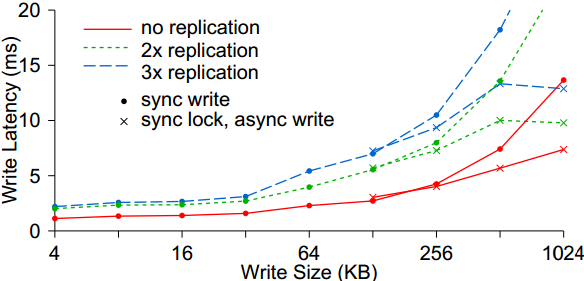
\includegraphics[width=\columnwidth]{p7.png} \\
  %Write latency, size and replication.
  \begin{enumerate}
   \item small writes minimal additional cost.
   \item large synchronous writes, transmission times dominate.
   \item Clients mask this latency for writes over 128K by acquring exclusive clocks.
  \end{enumerate}
 \end{columns}
\end{frame}

%\begin{frame}
% \frametitle{Write Latency}
% 
%\end{frame}

\begin{frame}
 \frametitle{Data Distribution and Scalability}
 \centering{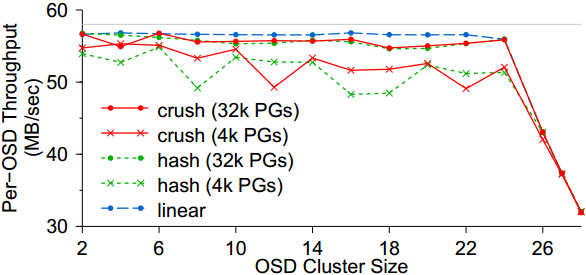
\includegraphics[width=0.7\textwidth]{p8.png}} \\
 \begin{itemize}
  \item OSD write performance scales linearly with the size of the OSD cluster.
  \item the saturated point is at 24 OSDs.
  \item more PGs and lower variance in OSD utilization can ease such situation.
 \end{itemize}
\end{frame}

\subsection{Metadata Performance}
\begin{frame}
 \frametitle{Metadata Update and Read Latency}
 \vspace{4pt}
 \centering{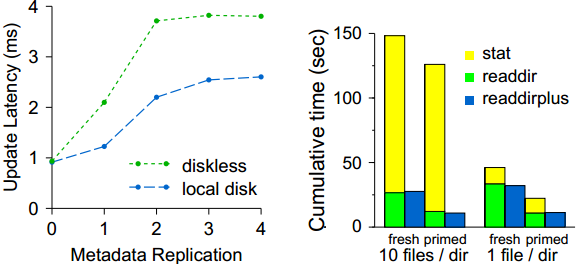
\includegraphics[width=0.7\textwidth]{p9.png} } \\
 left one: Metadata update latency, and the right one: the cumulative time. \\
 \begin{itemize}
  \item[*] Using a local disk lowers the write latency by avoiding the initial network round-trip.
  \item[**] Reads benefit from caching, and $readdirplus$ eliminate MDS interaction for $stats$ following $readdir$. 
 \end{itemize}
\end{frame}

\begin{frame}
 \frametitle{Metadata Scaling}
 \frametitle{OSD Throughput and Write Latency}
 \vspace{6pt}
 \begin{columns}[c]
    \column{0.5\textwidth}
  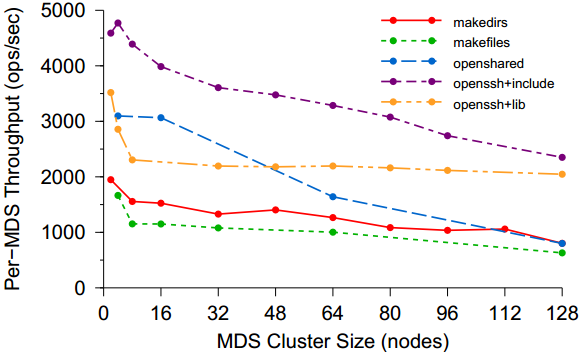
\includegraphics[width=\columnwidth]{p10.png} \\
  Per-MDS throughput, workloads and cluster sizes. \\
  \vspace{4pt}
  cluster grows to 128 nodes, efficiency $50\%$ below, and such issue allows vastly improved performance 
  over existing systems.
    \column{0.5\textwidth}
  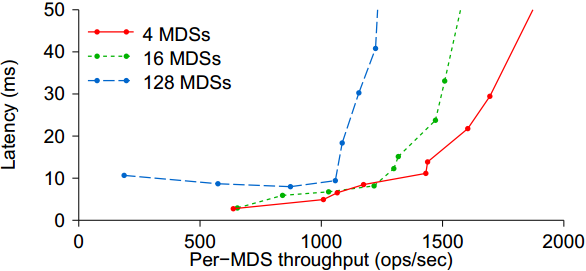
\includegraphics[width=\columnwidth]{p11.png} \\
  Average latency, per-MDS throughput and cluster sizes. \\
  \vspace{4pt}
  Large clusters have imperfect load distribution, resulting in lower average per-MDS throughput and 
  slightly higher latencies.
 \end{columns} 
\end{frame}


\section{Conclusion and Future work}
\begin{frame}
 \vspace{6pt}
 \textbf{Conclusion}:\\
 \begin{itemize}
  \item \textbf{Maximize} separate data from metadata management,scale \textbf{independently}, relies on CHRUSH.
  \item Ceph leverages \textbf{intelligent} OSDs to manage data replication, failure detection and recovery etc., good \textbf{performance}.
  \item Ceph's metadata management \textbf{architecture}, highly scalable storage, \textbf{dynamic subtree partition}.
 \end{itemize}
  \vspace{6pt}
  Apart from stated above, there are some points needed to be \textbf{enhanced}, eg. MDS failure recovery, 
  POSIX calls, MDS's ability to create snapshots of arbitrary subtrees, OSD's dynamic adjust the level of replication 
  based on the workloads, developing a QoS architecture and so on.
\end{frame}

%\begin{frame}
% \frametitle{存储效率和可靠性背景}
% \vspace{20pt}
% \begin{exampleblock}{背景}
%  随着分布式存储系统规模的不断扩大,系统可靠性的问题逐渐受到人们的重视。系统中磁盘数量的增加和单块磁盘容量的增长使得系统错误率不断增长,任何一次数据丢失都会造成巨大的损失。 \\
% \vspace{4pt}
%  可靠性是系统性能中的重要组成部分.对于存储系统而言,数据服务的可靠性是可靠性研究的核心.存储系统的可靠性描述了系统能有效地提供数据服务的能力,用系统能正常提供服务的概率表示.
% \end{exampleblock}
%\end{frame}

\frame{
 \frametitle{References}
 \vspace{24pt}
 \small{
 \begin{enumerate}[1]
  \item http://ceph.com/
  \item http://www.ibm.com/developerworks/linux/library/l-ceph/index.html?ca=dgr-lnxw01CEPHdth-LX
  \item http://deltamaster.is-programmer.com/posts/31908.html
  \item http://www.alidata.org/archives/1589
  \item http://blog.csdn.net/changtao381/article/details/8698935
  \item \ldots
 \end{enumerate}
}
}

\frame{
    \frametitle{Questions and answers}
    \begin{figure}
        
\includegraphics[width=6cm]{faq.jpg}
    \end{figure}
}

\end{CJK}
\end{document}
